\chapter{INTRODUCTION} \label{chap:intro}
In recent years, there has been a widespread increase in the use of GPUs in the field of machine learning and deep learning, because of their ability to massively speedup the training of models. This is mainly due to the large parallel processing ability of GPUs, which can process multiple inputs using SIMD intrinsics. Genetic Programming(GP) is an class of a machine algorithms with several inherent parallel steps. As such, it is an ideal domain for GPU based parallelization. 

\section{The Problem}
\label{intro:problem}
Genetic  Programming is a technique which involves evolving a set of programs based on the principles of genetics and natural selection. It is a generalize heuristic search technique, which searches for a least suitable program optimizing a given fitness function. 
As such it has applications ranging from machine learning to code synthesis.\citep{Koza92} It also supports a meta-evolutionary framework, where a GP system itself can be evolved using GP.\citep{schaul2010metalearning}

However, in practice, it is difficult to scale GP algorithms. Fitness evaluation of candidate programs in GP algorithms is a well-known bottleneck and there are multiple previous attempts to overcome this problem - either through parallelization of the evaluation step(\citep{10.1007/978-3-540-71605-1_9},\citep{baeta2021tensorgp},\citep{DEAP_JMLR2012},\citep{gplearn},\citep{staats2017tensorflow}), or by eliminating the need for fitness computations itself through careful initialization and controlled evolution.\citep{biles2001autonomous}

\section{Our Contributions}
\label{intro:contrib} 
In this thesis, we provide details about a parallelized version of the generational GP algorithm to the solve the problems of Symbolic Regression and Transformation. We use a stack-based GP algorithm for simplified program evaluation(inspired by \citep{perkis}). Our algorithm can also be used to train symbolic binary-classifiers, where the classifier's output corresponds to the estimated equation of the decision boundary. 

Our main contributions are listed below:
\begin{itemize}
  \item We parallelize the selection and evaluation step of the generational GP algorithm, by conducting parallel tounaments and fitness evaluation among candidate populations. 
  \item We introduce a prefix-tree based Array of Structures (AoS) representation for candidate programs, along with a method to evaluate all programs on a dataset using a thread-local device side stack with constrained size. 
  \item We also provide a new method to perform tournaments for program selection in parallel using random numbers generated inside the GPU. 
  \item We then benchmark the time taken for program evaluation by our algorithm against other standard libraries like gplearn\citep{gplearn} and TensorGP\citep{baeta2021tensorgp}. We provide a study of the effect of population size, dataset size and program length on the final time taken for training. We also show the results of executing our algorithm on the Airline Regression, Airfoil-Self Noise and Year MSD datasets, all taken from the UCI Machine Learning repository\citep{Dua:2019}.
\end{itemize}
The code for our algorithm is to be merged with the cuML library\citep{raschka2020machine}, which is a part of the RAPIDS suite of open source libraries maintained by Nvidia Corporation.

\section{Outline}
\label{intro:outline}

The rest of this thesis is structured in the following way. 
\begin{itemize}
  \item \Cref{chap:bgrw} introduces the generational GP algorithm in detail, with respect to the selection, mutation and evaluation steps. It also briefly talks about other existing GP libraries and the strategies used for program evaluation in them. 
  \item \Cref{chap:ourwork} contains implementation details about our algorithm for performing symbolic regression. Here, we examine the new algorithm in detail, and also talk about a few challenges encountered when trying to implement it using CUDA
  \item \Cref{chap:experiments} contains the results of various benchmarks run on our algorithm implementation and their speedups with respect to some standard GP libraries. It also contains information about the performance of our algorithm on $3$ standard datasets.
  \item \Cref{chap:conclusion} talks about future extensions and possible optimizations to the current algorithm, like support for custom user-defined functions in addition to the pre-defined function set.
\end{itemize}

% \begin{figure}[htp]
%   \centering
%   \begin{subfigure}{\textwidth}
%     \centering
%     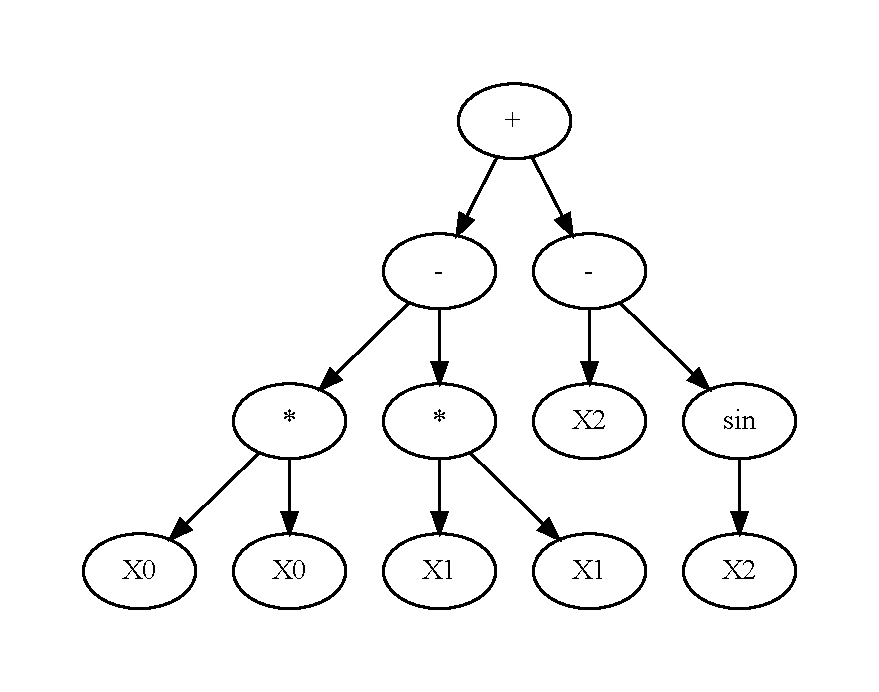
\includegraphics[scale=0.8]{images/graphviz/point_mut_before.dot.pdf}
%     \caption{The original expression tree}
%     \label{fig:point_muta}
%   \end{subfigure}%
%   \\
%   \begin{subfigure}{\textwidth}
%     \centering
%     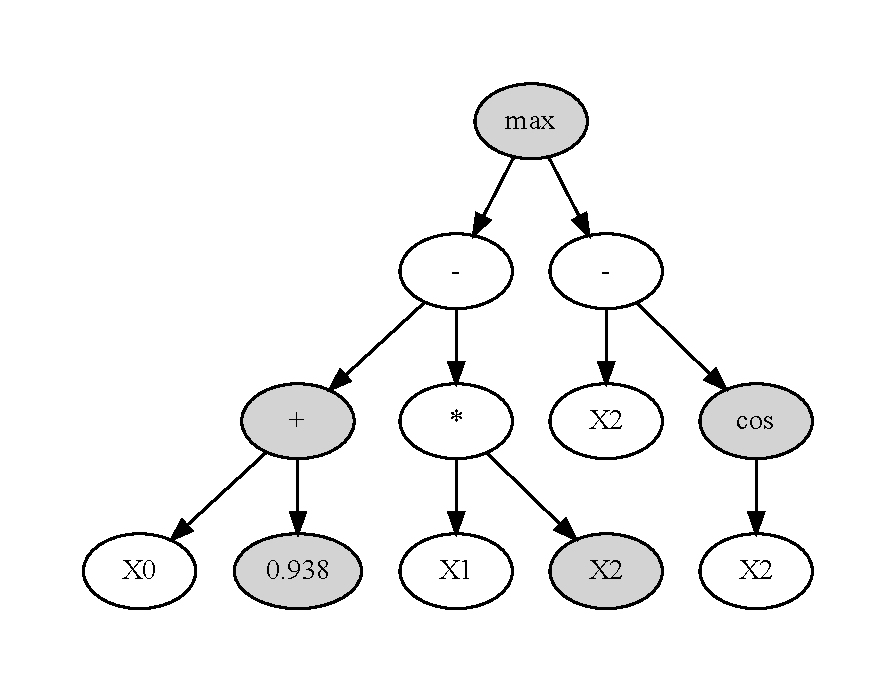
\includegraphics[scale=0.8]{images/graphviz/point_mut_after.dot.pdf}
%     \caption{The same expression tree after replacing some nodes(shaded here) with another node of the same arity}
%     \label{fig:point_mutb}
%   \end{subfigure}
%   \caption{Visualizing point mutations}
  
%   \label{fig:point_mut}
% \end{figure}

% \begin{figure}[htp]
%   \centering
%   \begin{subfigure}{\textwidth}
%     \raggedleft
%     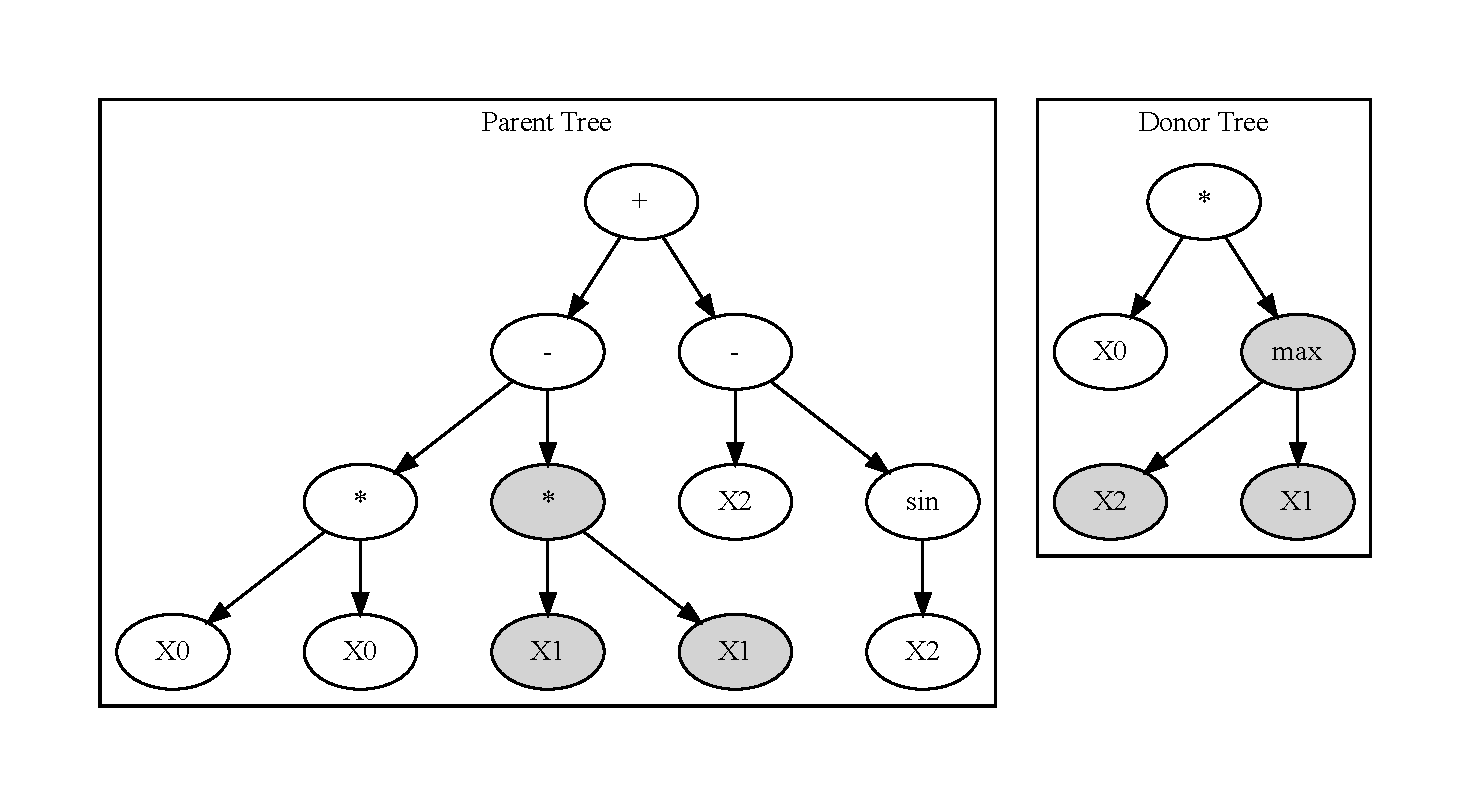
\includegraphics[scale=0.75]{images/graphviz/crossover_before.dot.pdf}
%     \caption{The original expression tree. The subtree to be hoisted is highlighted.}
%     \label{fig:hoist_muta}
%   \end{subfigure}%
%   \\
%   \begin{subfigure}{\textwidth}
%     \centering
%     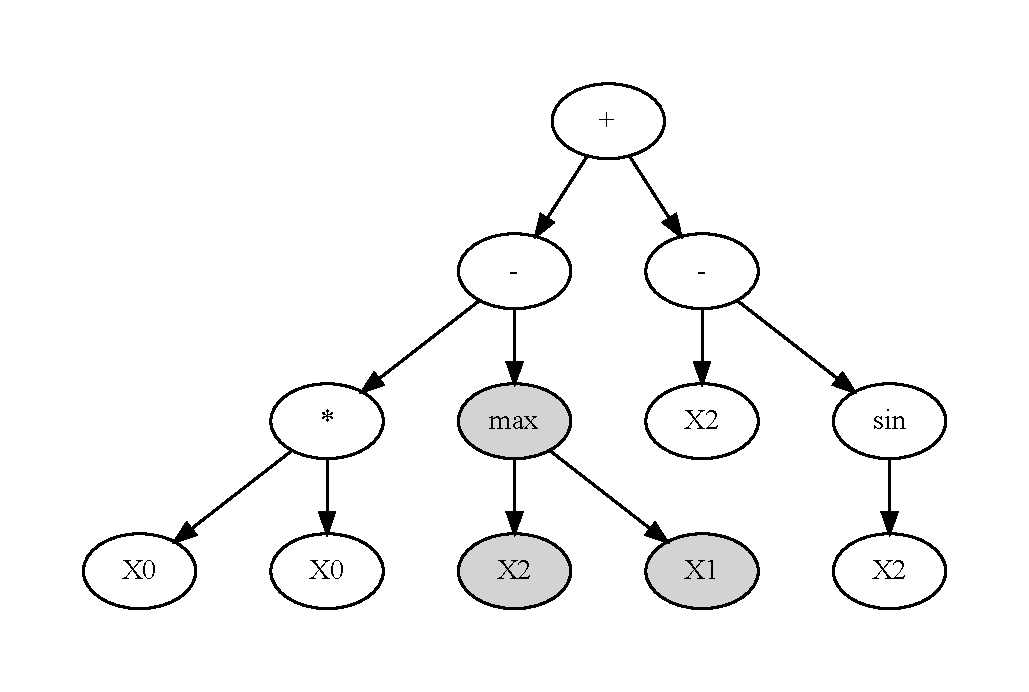
\includegraphics[scale=0.75]{images/graphviz/crossover_after.dot.pdf}
%     \caption{The same expression tree after hoisting the subtree}
%     \label{fig:hoist_mutb}
%   \end{subfigure}
%   \caption{Visualizing crossover mutations}
  
%   \label{fig:hoist_mut}
% \end{figure}

%  \begin{table}[htbp]
%    \caption{A sample table with a table caption placed
%      appropriately. This caption is also very long and is
%      single-spaced.  Also notice how the text is aligned.}
%    \begin{center}
%    \begin{tabular}[c]{|c|r|} \hline
%      $x$ & $x^2$ \\ \hline 
%      1  &  1   \\
%      2  &  4  \\
%      3  &  9  \\
%      4  &  16  \\
%      5  &  25  \\
%      6  &  36  \\
%      7  &  49  \\
%      8  &  64  \\ \hline
%    \end{tabular}
%    \label{tab:sample}
%    \end{center}
%  \end{table}